% --------------------------------------------------------------------------- %
\subsection{Диаграммы потоков данных}
% --------------------------------------------------------------------------- %
\begin{frame}
    \begin{itemize}
        \item Описание алгоритма представляет собой ориентированный граф.
        \item С его вершинами связываются процессы обработки данных.
        \item Его рёбра определяют пути данных между процессами.
    \end{itemize}

    \begin{figure}
        \centering
        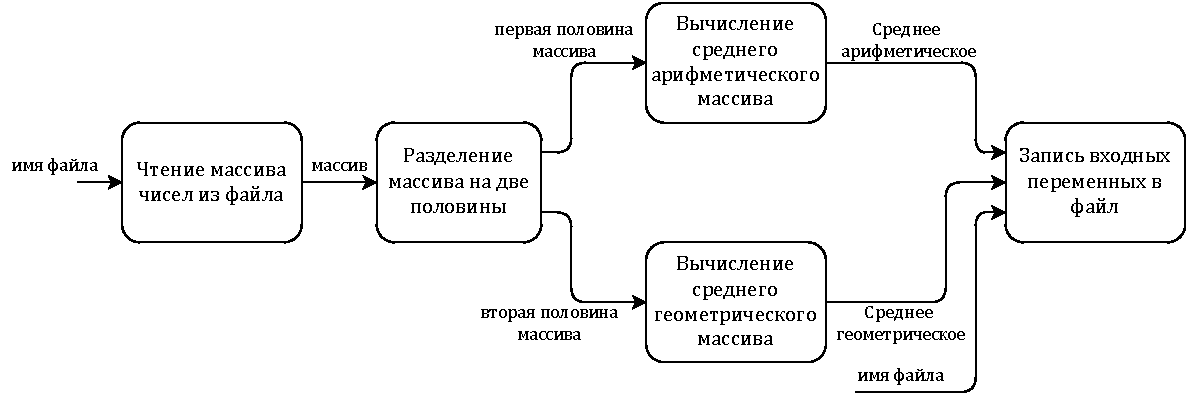
\includegraphics[width=0.9\textwidth]{images/illustration.dataflow.pdf}
        \caption{Пример диаграммы потоков данных, описывающей вычисление среднего арифметического и среднего геометрического двух половин массива целых чисел с последующей записью результатов в файл}
    \end{figure}

\end{frame}


\subsection{pSeven -- реализация диаграмм потоков данных}
%%%%%%%%%%%%%%%%%%%%%%%%%%%%%%%%%%%%%%%%%%%
\begin{frame}
    \begin{figure}
        \centering
        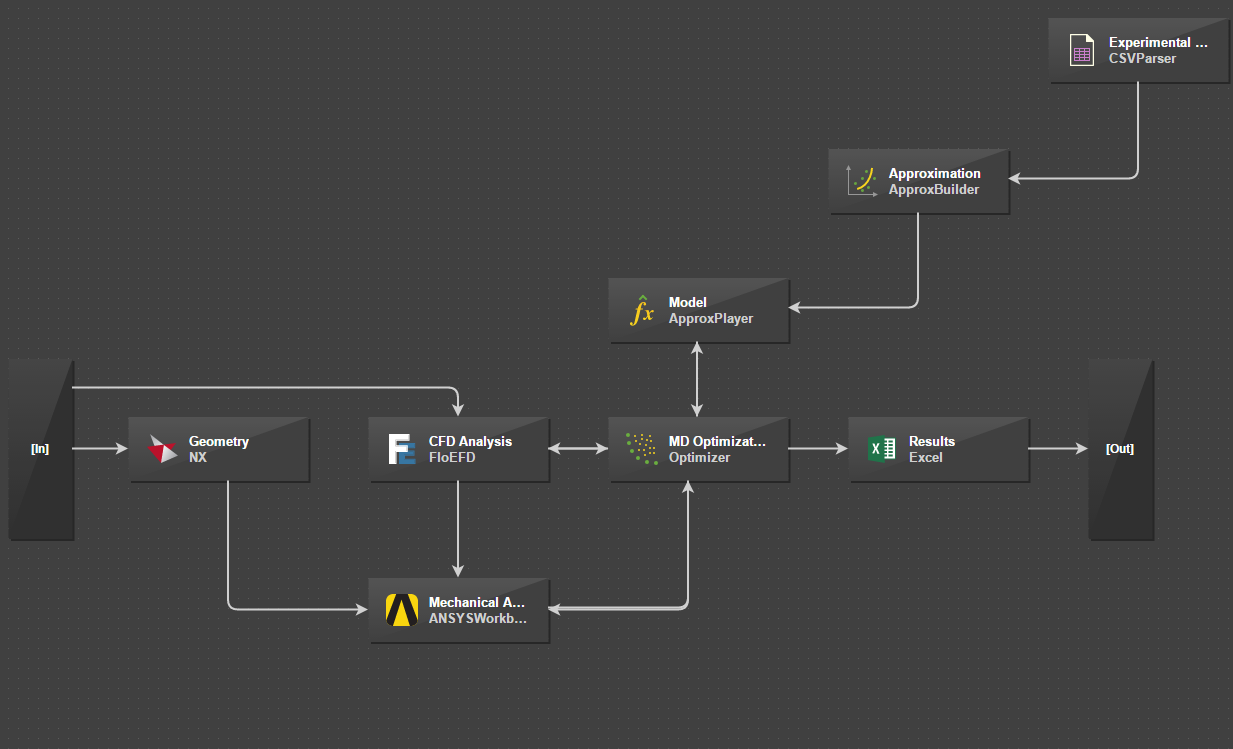
\includegraphics[width=\textwidth]{images/workflow1.png}
        \caption{Графический пользовательский интерфейс pSeven}
    \end{figure}

\end{frame}

% --------------------------------------------------------------------------- %
\subsection{Результаты сравнения. Выявленные достоинства объекта разработки}
% --------------------------------------------------------------------------- %
\begin{frame}
    Основные достоинства comsdk по сравнению с pSeven:
    \begin{itemize}
        \item Нет необходимости указывать входные и выходные данные при описании алгоритма.
        \item По умолчанию поддерживаются алгоритмы, подразумевающие взаимодействие с пользователем
    \end{itemize}

    \begin{figure}
        \centering
        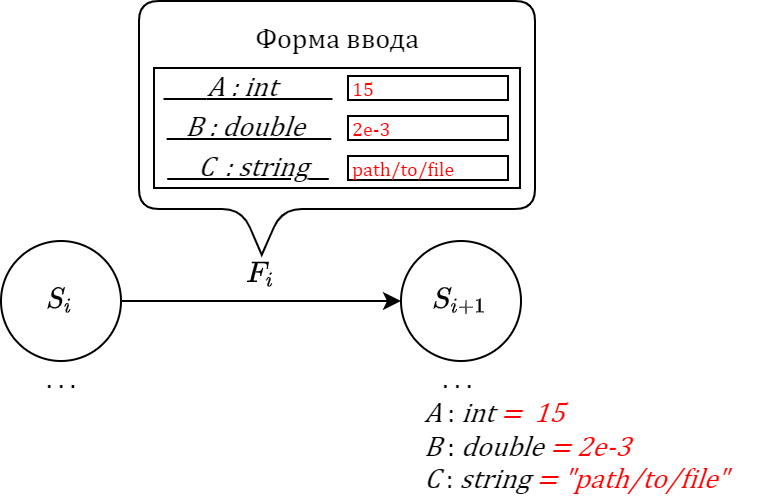
\includegraphics[height=0.33\textheight]{images/illustration.form_generation.png}
        \caption{Пример получения данных от пользователя при помощи генерируемой формы ввода}
    \end{figure}

    \begin{itemize}
        \item Результат применения -- компилируемая программа с возможностью запуска на различных платформах.
    \end{itemize}
\end{frame}

% --------------------------------------------------------------------------- %
\subsection{Результаты сравнения. Выявленные недостатки объекта разработки}
% --------------------------------------------------------------------------- %
\begin{frame}
    Основные недостатки comsdk по сравнению с pSeven:
    \begin{itemize}
        \item Отсутствие поддержки матричных типов данных.
        \item Отсутствие средств визуализации результатов расчётов.
        \item Отсутствие возможности использования при расчётах распределённых вычислительных систем;
    \end{itemize}
\end{frame}

% --------------------------------------------------------------------------- %
\subsection{Цели и задачи разработки}
% --------------------------------------------------------------------------- %
\begin{frame}

    \begin{block}{Цель}
        Разработать обновлённые программные средства для создания и интерпретации графовых описаний вычислительных методов в программном каркасе comsdk.
    \end{block}

    \begin{block}{Задачи}
        \begin{enumerate}
            \item Сформировать требования к алгоритму, выполняющему этапы алгоритма по его описанию, составленному по методологии GBSE.
            \item Спроектировать структуры данных для описания и представления описаний алгоритмов и их элементов в программном каркасе comsdk.
            \item Разработать алгоритм обхода графовых моделей с использованием спроектированных структур данных.
            \item Представить интерфейсы или реализации разработанных алгоритмов и структур данных на языке С++.
        \end{enumerate}
    \end{block}

\end{frame}